\documentclass[]{article}

\usepackage{amsmath, amssymb} % Math formatting and symbols
\usepackage{graphicx} % Insert graphics
\usepackage{wrapfig} % Allow text to wrap around images
\usepackage[cm]{fullpage} % Smaller margins and header/footer
\usepackage{setspace}
\usepackage{gensymb} % degree symbol

\usepackage{enumitem} % Allow for widest tag in enumerate

\renewcommand*\descriptionlabel[1]{\hspace\leftmargin$#1$}

\newenvironment{adescription}[1]
{\begin{list}{}%
		{\renewcommand\makelabel[1]{##1\hfill}%
			\settowidth\labelwidth{\makelabel{#1}}%
			\setlength\leftmargin{\labelwidth}
			\addtolength\leftmargin{\labelsep}}}
	{\end{list}}

\newcommand{\bd}{\textbf}
\newcommand{\dquad}{\quad{}\quad{}}

\title{Legislative Branch \& Elections}
\author{}
\date{}

\begin{document}

\maketitle

\subsection*{US Congress}
-- 535 members

\begin{wrapfigure}{r}{0.55\textwidth}
	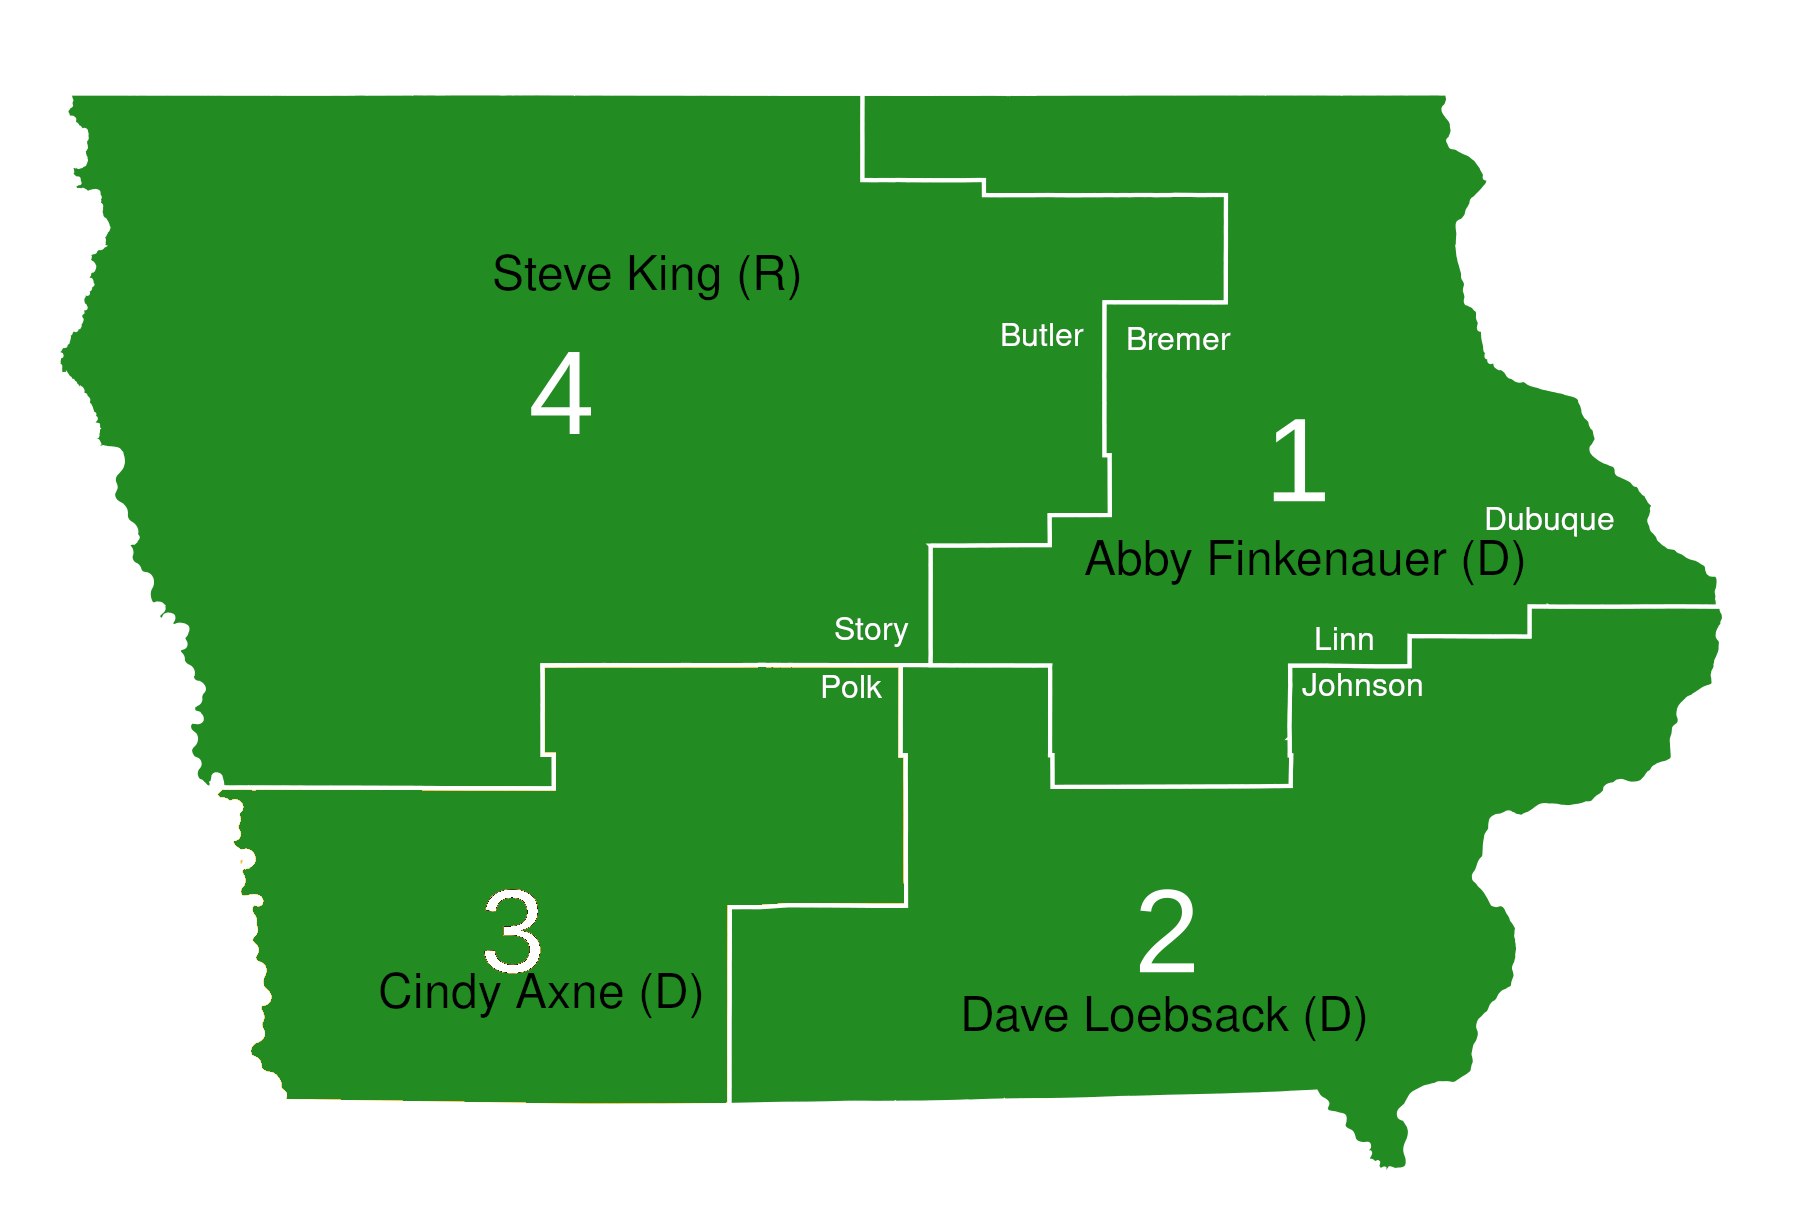
\includegraphics[width=1.1\linewidth]{iowa-districts.png}
	\caption{Iowa's Congressional Districts}
\end{wrapfigure}

\subsection*{Senators}
-- 100 members (\emph{2 per state}) \\
-- 30+ years old \\
-- 6 year term, Why? \\
\indent-- Stability

\subsection*{House of Representatives}
-- 435 members (\emph{Based on population, $1 \approx 700000$}) \\
-- 25+ years old \\
-- 2 year term, Why? \\
\indent-- ???

\subsection*{Iowa}
	\subsubsection*{Senators}
		\begin{itemize}
			\item Charles (Chuck) Grassley (R) (\emph{Senior Senator})
			\item Joni Ernst (R) (\emph{Junior Senator})
		\end{itemize}
	\subsubsection*{Representatives (\emph{by district})}
		\begin{enumerate}
			\item Abby Finkenauer (D)
			\item Dave Loebsack (D)
			\item Cindy Axne (D)
			\item Steve King (R)
		\end{enumerate}

\end{document}
